\documentclass{article}
\usepackage[utf8]{inputenc}
\usepackage[italian]{babel}
\usepackage{graphicx}

\title{Studio del comportamento di un circuito RC serie
in regime di corrente alternata mediante
simulazione con LTSpice}
\author{O. D. Caputo, C. Crismale, E. Panteghini}
\date{~}

\begin{document}

\maketitle

\section{Illustrazione della teoria di base}
Quando messi in regime di corrente alternata, i circuiti RC in serie si comportano come dei filtri di frequenza, ovvero permettono il passaggio di corrente solo a certe frequenze, in relazione
a dove le misure vengono effettuate; il filtro è definito “passa basso”
quando la misura viene effettuata ai capi del condensatore, mentre è detto “passa
alto” quando la misura viene effettuata ai capi del resistore. Come si evince dalla
denominazione, un filtro di tipo “passa alto” attenua tutte le pulsazioni al di
sotto di una $\omega_0$, viceversa, un filtro “passa basso” attenua le pulsazioni al di
sopra di $\omega_0$. Il valore $\omega_0$ è detto “frequenza o pulsazione di taglio” e si
calcola come: $\omega_0 = \frac{1}{RC}$ . Mentre ovviamente la frequenza $f$ è data da $f = \frac{\omega}
{2\pi}$
I comportamenti dei ciruciti vengono studiati mediante i diagrammi
di Bode, grafici in cui possiamo rappresentare in funzione della frequenza del segnale, il guadagno tra tensione in ingresso e in uscita sull’elemento circuitale in scala logaritmica, oppure
l’andamento dello sfasamento tra il segnale in ingresso e quello in uscita. In particolare, chiamato $G_r$ il guadagno ai
capi del resistore, $G_c$ guadagno ai capi del condensatore, entrambi in decibel e
$\varphi$ lo sfasamento, in gradi, tra segnale erogato dal generatore e quello ai capi di uno dei 2 elementi circuitali,  risulta che:
\begin{equation}
    G_r = -10\log_{10}{\Bigl( 1 + \frac{\omega_0^2}{\omega^2}\Bigl)}
\end{equation}
\begin{equation}
     G_c = -10\log_{10}{\Bigl( 1 + \frac{\omega_0^2}{\omega^2}\Bigl)}
\end{equation}
\begin{equation}
    \varphi = \frac{\pi}{180} \Bigl( 2\pi \frac{\Delta T}{T} \Bigl)
\end{equation}

\begin{figure}
    \centering
    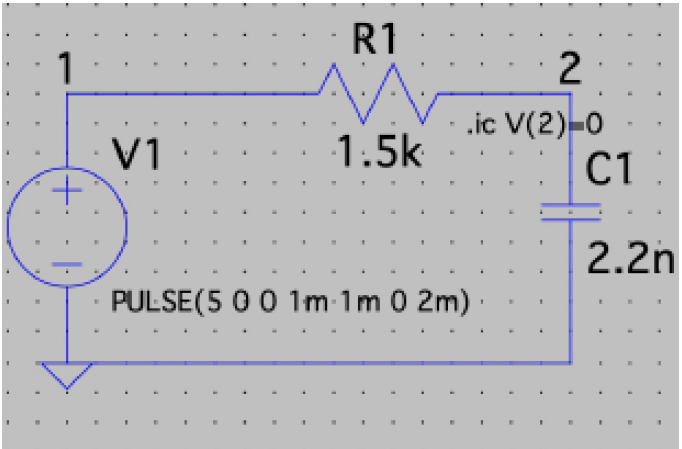
\includegraphics[width=\linewidth]{figure1.png}
    \caption{Circuito simulato sul programma \emph{LTSpice}, con generatore in modalità PULSE}
    \label{figura1}
\end{figure}

\noindent ove $\Delta T$ è la differenza tra i periodi dei 2 segnali e T è il periodo del segnale in
entrata. \\
Inoltre è stato possibile mediante la Trasformata di Fourier, analizzare il comportamento del circuito quando veniva fornito un segnale di onda quadra in ingresso. Questo strumento
matematico consente lo sviluppo di una qualsiasi funzione periodica, in
questo caso la funzione che rappresentava l’onda quadra in analisi, attraverso
una combinazione lineare di funzioni seno e coseno secondo:
\begin{equation}
    f(t) = \frac{a_0}{2} + \sum_{n=1}^{\infty}{a_n \cos(\omega nt)} + \sum_{n=1}^{\infty}{b_n \sin(\omega nt)}
\end{equation}
ove
\begin{equation}
    a_0 = \frac{2}{T}\int_{0}^{T}f(t)dt
\end{equation}
\begin{equation}
    a_n = \frac{2}{T}\int_{0}^{T}f(t)\cos(\omega nt)dt
\end{equation}
\begin{equation}
    b_n = \frac{2}{T}\int_{0}^{T}f(t)\sin(\omega nt)dt
\end{equation}
\section{Illustrazione del metodo di misura e della strumentazione}
\subsection{Strumentazione dell'esperimento}
Attraverso il simulatore di circuiti lineari \emph{LTSpice}, si è potuto simulare un
circuito RC con generatore di tensione alternata oppure a gradini.
In particolare si è simulato:
\begin{itemize}
    \item[-] n.1 resistore (1,5 $k\Omega$)
    \item[-] n.1 condensatore (2.2 nF)
    \item[-] n.1 generatore di tensione impostabile in modalità SINE (tensione alternata) e PULSE (tensione a gradini).
\end{itemize}
Per le misure, il programma consente la visualizzazione delle tensioni
tra 2 punti del circuito come se si usasse un oscilloscopio digitale.

\subsection{Metodo di misura}
L’analisi del circuito è stata eseguita usando il programma di simulazione di
circuiti lineari \emph{LTSpice}. Dal catalogo presente nel simulatore, è stato scelto un generatore di tensione con possibilità di scegliere una tensione alternata e, in
seguito, un’onda quadra. Inoltre si sono scelti resistore e condensatore presenti nella barra di lavoro del programma, impostati ripettivamente a 1.5 $k\Omega$ e 2.2nF. Costruito il circuito in serie RC, si sono usate due direttive diverse:
\begin{itemize}
    \item[-] \emph{.tran} che permette la simulazione dell’evoluzione della tensione in funzione del tempo
    \item[-] \emph{.ac dec 101 10 100Meg} che permette la simulazione di guadagno e sfasamento del segnale in entrata e quello ai capi dell’elemento selezionato, potendo così ottenere i diagrammi di Bode. Mentre per il generatore si è scelta l’opzione SINE per la simulazione di una tensione alternata di 20V, mentre PULSE per la simulazione dell’onda quadra.
\end{itemize}

\section{Presentazione dei risultati}
Per quanto concerne i risultati relativi al filtro passa basso è stato possibile
calcolare il rapporto tra le ampiezze (ossia il guadagno) e lo sfasamento dei
segnali rispetto al segnale di ingresso: come si può osservare dai grafici, le
tensioni ai capi dei due filtri dipendono dalla frequenza dell’onda in ingresso. Di
seguito, si riportano i valori ottenuti per rapporto fra le ampiezze e sfasamento
per ciascun valore della frequenza considerato:
\subsection{f = 500Hz}
Applicando una sollecitazione con frequenza di 500 Hz, per il filtro passa alto si
è potuta osservare una ingente diminuzione del segnale con conseguente sfasamento.
Si sono misurate un’ampiezza del segnale pari a $ V_r = (0.21 \pm 0.05) V$ ed una differenza del periodo $\Delta T = (0.50 \pm 0.05) ms$. pertanto, il rapporto tra le
ampiezze risulta essere pari a $\frac{V_r}{\varepsilon_0}
=0.21V/20V=0.010$, dove $\varepsilon_0$ indica l’ampiezza
della tensione in entrata. Di conseguenza, lo sfasamento risulta essere pari a:
\begin{equation}
    \varphi = \Bigl ( 2\pi \frac{\Delta T}{T} \Bigl) \frac{180}{\pi} = 90.00 \pm 0.05
\end{equation}
ove la grandezza è espressa in gradi sesagesimali. Invece, per il filtro passa basso
il rapporto calcolato risulta essere pari a 1, in fase con il segnale in uscita.


\subsection{f = 50kHz}
In questo caso, per il filtro passa alto si è misurata un’ampiezza $V_r = (14.4 \pm 1) V$, il quale fornisce un guadagno pari a $\frac{V_r}{\varepsilon_0} = 0.720$; tale risultato è compatibile
con quello previsto, in quanto si tratta di un valore prossimo alla frequenza di
taglio, il cui valore nominale è pari a f = 48 kHz. La differenza dei periodi ha
un valore corrispondente a $\Delta T = 3.50 \mu s$, al quale corrisponde una differenza di
fase pari a $\varphi =45.0$. Si ottengono valori simili per il filtro passa basso: infatti, l’ampiezza risulta essere $V_r = 14.14 V$ con una differenza tra i periodi di $\Delta T =
(3.60 \pm 0.05) \mu s$; di conseguenza, il rapporto fra le ampiezze è $\frac{V_r}{\varepsilon_0} = 0.707$ e la
differenza di fase associata è pari a $\varphi= 45.00$\footnote{Le differenze di fase sono in gradi sessagesimali}
\begin{figure}
    \centering
    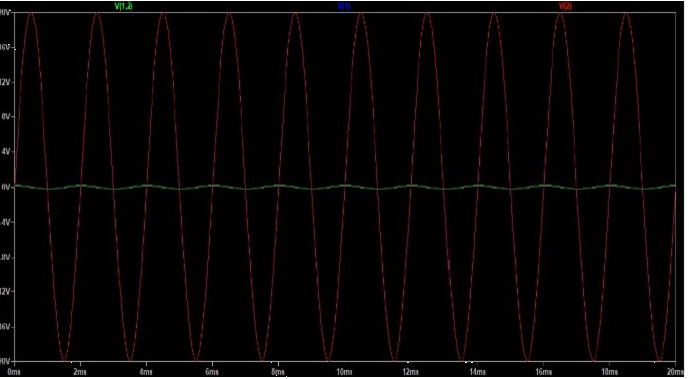
\includegraphics[width=\linewidth]{figure2.png}
    \caption{Tensione ai capi degli elementi circuitali: in rosso il segnale fornito dal generatore, in verde ai capi del resistore, in blu ai capi di C a 500Hz}
    \label{figura2}
\end{figure}

\subsection{f = 500kHz}
Trattandosi di un segnale avente frequenza molto maggiore rispetto a quella di
taglio, si osserva che per il filtro passa alto lo sfasamento è pressoché nullo e,
quindi, il rapporto fra le frequenze tende a 1. Invece, per quanto riguarda il filtro
passa basso la differenza di periodo è pari a $\Delta t = 0.50 ms$, alla quale è associato uno sfasamento dato da $\varphi = 90.00^{\circ} \pm 0.052$\footnote{Le differenze di fase sono in gradi sessagesimali}; invece, l’ampiezza del segnale ha un
valore pari a $V_r = 2.0 V$, da cui si ottiene il rapporto corrispondente a $\frac{V_r}{\varepsilon_0} = 0.1$.
\begin{figure}
    \centering
    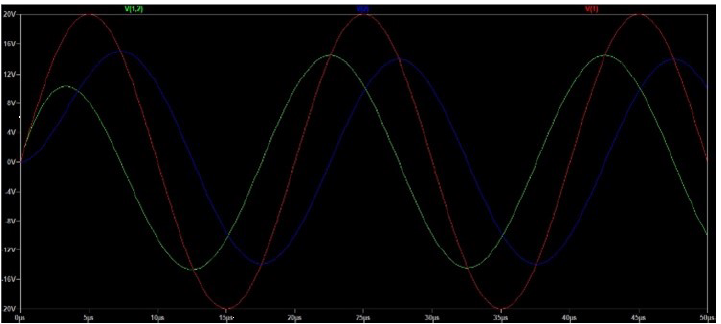
\includegraphics[width=\linewidth]{figure3.png}
    \caption{Tensione ai capi degli elementi circuitali: in rosso il segnale fornito dal generatore, in verde ai capi del resistore, in blu ai capi di C a 50kHz}
    \label{figura3}
\end{figure}
\begin{figure}
    \centering
    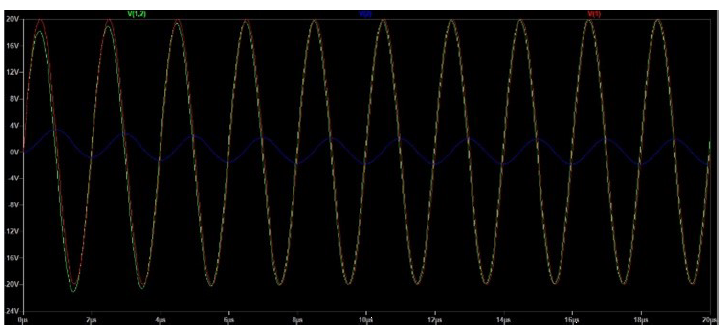
\includegraphics[width=\linewidth]{figure4.png}
    \caption{Tensione ai capi degli elementi circuitali: in rosso il segnale fornito dal generatore, in verde ai capi del resistore, in blu ai capi di C a 500kHz}
    \label{figura4}
\end{figure}
\subsection{Analisi dei diagrammi di Bode}
Un’ulteriore analisi è stata effettuata tramite i diagrammi di Bode, ovvero grafici
che rappresentano in funzione del tempo il guadagno di un segnale, espresso in decibel, e l’andamento
dello sfasamento di quest’ultimo. Successivamente,
si è effettuata l'interpolazione dei dati, che presentano un andamento
lineare: quindi, si è ottenuta una retta, come si evince dai grafici sotto riportati
(figure 5 e 6), da cui è stato possibile ricavare il valore della frequenza
di taglio; in particolare, per il filtro passa alto si è ottenuta una frequenza
pari a $f_T = 47 kHz$ e per il filtro passa basso $f_T= 49 kHz$. Inoltre, i valori
del guadagno per ciascuno é, rispettivamente, G =-3.10 dB e G =-2.92 dB,
compatibili con il valore teorico pari a G = -3 dB.
\begin{figure}[h!]
    \centering
    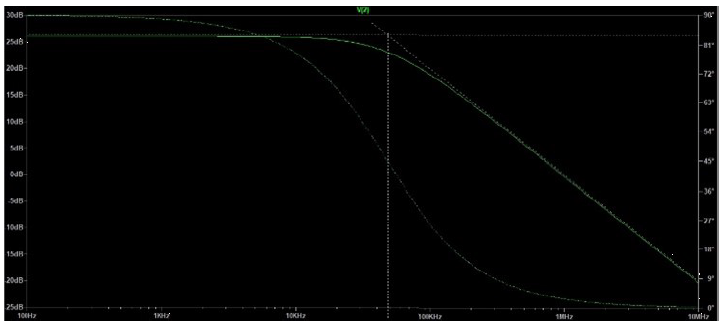
\includegraphics[width=\linewidth]{figure5.png}
    \caption{Diagrammi di Bode ai capi di C}
    \label{figura5}
\end{figure}
\begin{figure}[h!]
    \centering
    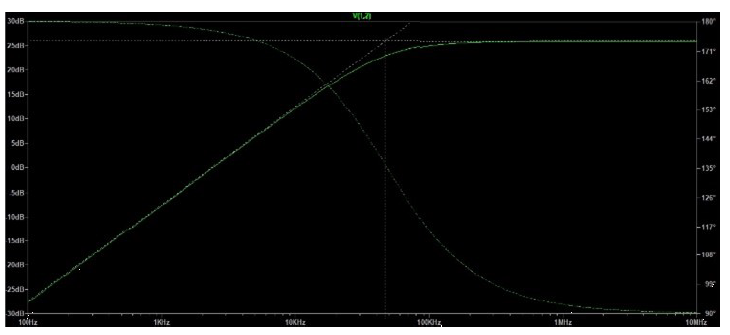
\includegraphics[width=\linewidth]{figure6.png}
    \caption{Diagrammi di Bode ai capi di R}
    \label{figura6}
\end{figure}
\subsection{Analisi dell'onda quadra}
Infine, si è effettuata l’analisi dell’onda quadra in ingresso, la quale presenta
un’ampiezza pari a $V_r = 5 V$ e periodo T = 10 ms. Mediante gli strumenti in
dotazione di \emph{LTSpice} è stato possibile graficare tensione del generatore (simulando
un generatore di funzioni che eroga un’onda quadra), tensione ai capi di
R e tensione ai capi di C, come se si avesse a disposizione un oscilloscopio.
\subsection{Nota agli errori e incertezze}
Naturalmente trattandosi di una simulazione di un circuito, essa sarà priva di incertezze sperimentali. Tuttavia, risulta logico che in un’esperienza
reale ogni dato è soggetto a errori di natura statistica e sistematica. In particolare;
per effettuare la misura e ricreare tale esperienza è utile usare un oscilloscopio
digitale. L’incertezza sui dati viene ottenuta considerando la semiampiezza della
tacca più piccola sullo schermo dello strumento, che indica anche le unità di
misura e scala regolabili in base al segnale. Per le grandezze rerivate è possibile
propagare l’incertezza mediante la nota relazione di propagazione degli errori.

\begin{figure}
    \centering
    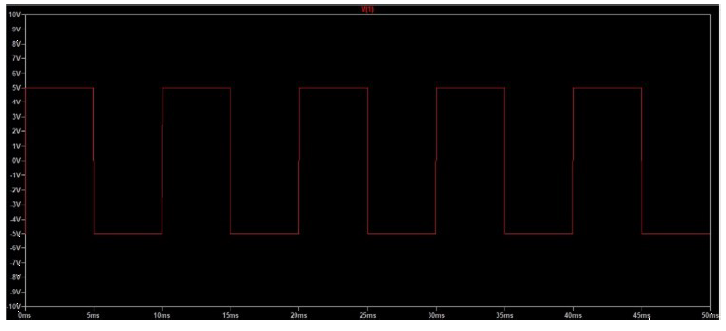
\includegraphics[width=\linewidth]{figure7.png}
    \caption{Tensione al variare del tempo erogata dal generatore usando un generatore di onde quadre - comando PULSE}
    \label{figura7}
\end{figure}
\begin{figure}
    \centering
    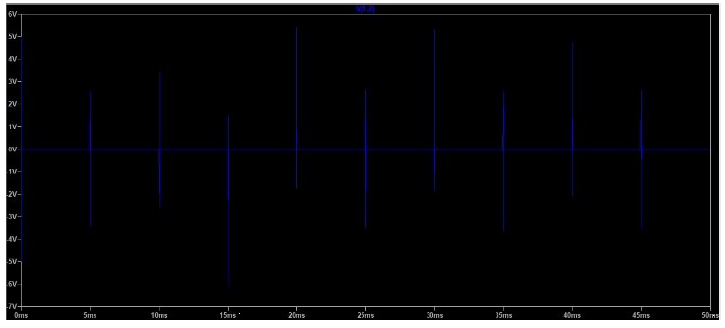
\includegraphics[width=\linewidth]{figure8.png}
    \caption{Tensione al variare del tempo ai capi della resistenza quando viene
erogata dal generatore un’onda quadra - comando PULSE}
    \label{figura8}
\end{figure}
\begin{figure}
    \centering
    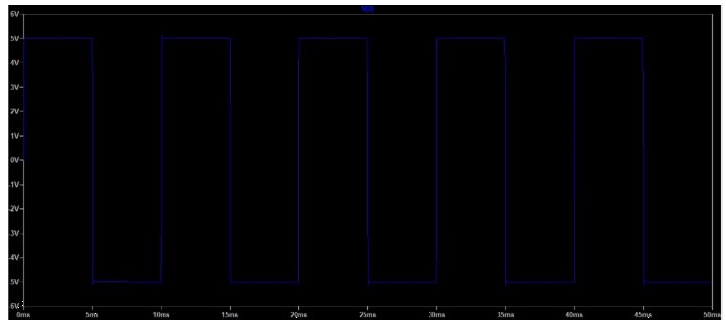
\includegraphics[width=\linewidth]{figure9.png}
    \caption{Tensione al variare del tempo ai capi del condensatore quando viene
erogata dal generatore un’onda quadra - comando PULSE}
    \label{figura9}
\end{figure}

\end{document}